% Lines starting with a percent sign (%) are comments. LaTeX will 
% not process those lines. Similarly, everything after a percent 
% sign in a line is considered a comment. To produce a percent sign
% in the output, write \% (backslash followed by the percent sign). 
% ==================================================================
% Usage instructions:
% ------------------------------------------------------------------
% The file is heavily commented so that you know what the various
% commands do. Feel free to remove any comments you don't need from
% your own copy. When redistributing the example thesis file, please
% retain all the comments for the benefit of other thesis writers! 
% ==================================================================
% Compilation instructions: 
% ------------------------------------------------------------------
% Use pdflatex to compile! Input images are expected as PDF files.
% Example compilation:
% ------------------------------------------------------------------
% > pdflatex thesis-example.tex
% > bibtex thesis-example
% > pdflatex thesis-example.tex
% > pdflatex thesis-example.tex
% ------------------------------------------------------------------
% You need to run pdflatex multiple times so that all the cross-references
% are fixed. pdflatex will tell you if you need to re-run it (a warning
% will be issued)  
% ------------------------------------------------------------------
% Compilation has been tested to work in ukk.cs.hut.fi and kosh.hut.fi
% - if you have problems of missing .sty -files, then the local LaTeX
% environment does not have all the required packages installed.
% For example, when compiling in vipunen.hut.fi, you get an error that
% tikz.sty is missing - in this case you must either compile somewhere
% else, or you cannot use TikZ graphics in your thesis and must therefore
% remove or comment out the tikz package and all the tikz definitions. 
% ------------------------------------------------------------------

% General information
% ==================================================================
% Package documentation:
% 
% The comments often refer to package documentation. (Almost) all LaTeX
% packages have documentation accompanying them, so you can read the
% package documentation for further information. When a package 'xxx' is
% installed to your local LaTeX environment (the document compiles
% when you have \usepackage{xxx} and LaTeX does not complain), you can 
% find the documentation somewhere in the local LaTeX texmf directory
% hierarchy. In ukk.cs.hut.fi, this is /usr/texlive/2008/texmf-dist,
% and the documentation for the titlesec package (for example) can be 
% found at /usr/texlive/2008/texmf-dist/doc/latex/titlesec/titlesec.pdf.
% Most often the documentation is located as a PDF file in 
% /usr/texlive/2008/texmf-dist/doc/latex/xxx, where xxx is the package name; 
% however, documentation for TikZ is in
% /usr/texlive/2008/texmf-dist/doc/latex/generic/pgf/pgfmanual.pdf
% (this is because TikZ is a front-end for PGF, which is meant to be a 
% generic portable graphics format for LaTeX).
% You can try to look for the package manual using the ``find'' shell
% command in Linux machines; the find databases are up-to-date at least
% in ukk.cs.hut.fi. Just type ``find xxx'', where xxx is the package
% name, and you should find a documentation file.
% Note that in some packages, the documentation is in the DVI file
% format. In this case, you can copy the DVI file to your home directory,
% and convert it to PDF with the dvipdfm command (or you can read the
% DVI file directly with a DVI viewer).
% 
% If you can't find the documentation for a package, just try Googling
% for ``latex packagename''; most often you can get a direct link to the
% package manual in PDF format.
% ------------------------------------------------------------------


% Document class for the thesis is report
% ------------------------------------------------------------------
% You can change this but do so at your own risk - it may break other things.
% Note that the option pdftext is used for pdflatex; there is no
% pdflatex option. 
% ------------------------------------------------------------------
\documentclass[12pt,a4paper,oneside,pdftex]{report}

% The input files (tex files) are encoded with the latin-1 encoding 
% (ISO-8859-1 works). Change the latin1-option if you use UTF8 
% (at some point LaTeX did not work with UTF8, but I'm not sure
% what the current situation is) 
\usepackage[latin1]{inputenc}
% OT1 font encoding seems to work better than T1. Check the rendered
% PDF file to see if the fonts are encoded properly as vectors (instead
% of rendered bitmaps). You can do this by zooming very close to any letter 
% - if the letter is shown pixelated, you should change this setting 
% (try commenting out the entire line, for example).  
\usepackage[OT1]{fontenc}
% The babel package provides hyphenating instructions for LaTeX. Give
% the languages you wish to use in your thesis as options to the babel
% package (as shown below). You can remove any language you are not
% going to use.
% Examples of valid language codes: english (or USenglish), british, 
% finnish, swedish; and so on.
\usepackage[finnish,swedish,english]{babel}


% Font selection
% ------------------------------------------------------------------
% The default LaTeX font is a very good font for rendering your 
% thesis. It is a very professional font, which will always be 
% accepted. 
% If you, however, wish to spicen up your thesis, you can try out
% these font variants by uncommenting one of the following lines
% (or by finding another font package). The fonts shown here are 
% all fonts that you could use in your thesis (not too silly). 
% Changing the font causes the layouts to shift a bit; you many
% need to manually adjust some layouts. Check the warning messages
% LaTeX gives you.
% ------------------------------------------------------------------
% To find another font, check out the font catalogue from
% http://www.tug.dk/FontCatalogue/mathfonts.html
% This link points to the list of fonts that support maths, but
% that's a fairly important point for master's theses.
% ------------------------------------------------------------------
% <rant>
% Remember, there is no excuse to use Comic Sans, ever, in any
% situation! (Well, maybe in speech bubbles in comics, but there 
% are better options for those too)
% </rant>

% \usepackage{palatino}
% \usepackage{tgpagella}



\usepackage{graphicx}
\usepackage{lineno}
\usepackage{float}


% Optional packages
% ------------------------------------------------------------------
% Select those packages that you need for your thesis. You may delete
% or comment the rest.

% Natbib allows you to select the format of the bibliography references.
% The first example uses numbered citations: 
\usepackage[square,sort&compress,numbers]{natbib}
% The second example uses author-year citations.
% If you use author-year citations, change the bibliography style (below); 
% acm style does not work with author-year citations.
% Also, you should use \citet (cite in text) when you wish to refer
% to the author directly (\citet{blaablaa} said blaa blaa), and 
% \citep when you wish to refer similarly than with numbered citations
% (It has been said that blaa blaa~\citep{blaablaa}).
% \usepackage[square]{natbib}

% The alltt package provides an all-teletype environment that acts
% like verbatim but you can use LaTeX commands in it. Uncomment if 
% you want to use this environment. 
% \usepackage{alltt}

% The eurosym package provides a euro symbol. Use with \euro{}
\usepackage{eurosym} 

% Verbatim provides a standard teletype environment that renderes
% the text exactly as written in the tex file. Useful for code
% snippets (although you can also use the listings package to get
% automatic code formatting). 
\usepackage{verbatim}

% The listing package provides automatic code formatting utilities
% so that you can copy-paste code examples and have them rendered
% nicely. See the package documentation for details.
% \usepackage{listings}

% The fancuvrb package provides fancier verbatim environments 
% (you can, for example, put borders around the verbatim text area
% and so on). See package for details.
% \usepackage{fancyvrb}

% Supertabular provides a tabular environment that can span multiple 
% pages. 
%\usepackage{supertabular}
% Longtable provides a tabular environment that can span multiple 
% pages. This is used in the example acronyms file. 
\usepackage{longtable}

% The fancyhdr package allows you to set your the page headers 
% manually, and allows you to add separator lines and so on. 
% Check the package documentation. 
% \usepackage{fancyhdr}

% Subfigure package allows you to use subfigures (i.e. many subfigures
% within one figure environment). These can have different labels and
% they are numbered automatically. Check the package documentation. 
\usepackage{subfigure}
%\usepackage{subcaption}
\usepackage{graphicx}
\usepackage{caption}

% The titlesec package can be used to alter the look of the titles 
% of sections, chapters, and so on. This example uses the ``medium'' 
% package option which sets the titles to a medium size, making them
% a bit smaller than what is the default. You can fine-tune the 
% title fonts and sizes by using the package options. See the package
% documentation.
\usepackage[medium]{titlesec}

% The TikZ package allows you to create professional technical figures.
% The learning curve is quite steep, but it is definitely worth it if 
% you wish to have really good-looking technical figures. 
\usepackage{tikz}
% You also need to specify which TikZ libraries you use
\usetikzlibrary{positioning}
\usetikzlibrary{calc}
\usetikzlibrary{arrows}
\usetikzlibrary{decorations.pathmorphing,decorations.markings}
\usetikzlibrary{shapes}
\usetikzlibrary{patterns}

% The aalto-thesis package provides typesetting instructions for the
% standard master's thesis parts (abstracts, front page, and so on)
% Load this package second-to-last, just before the hyperref package.
% Options that you can use: 
%   mydraft - renders the thesis in draft mode. 
%             Do not use for the final version. 
%   doublenumbering - [optional] number the first pages of the thesis
%                     with roman numerals (i, ii, iii, ...); and start
%                     arabic numbering (1, 2, 3, ...) only on the 
%                     first page of the first chapter
%   twoinstructors  - changes the title of instructors to plural form
%   twosupervisors  - changes the title of supervisors to plural form
\usepackage[mydraft,twosupervisors]{aalto-thesis}
%\usepackage[mydraft,doublenumbering]{aalto-thesis}
%\usepackage{aalto-thesis}


% Hyperref
% ------------------------------------------------------------------
% Hyperref creates links from URLs, for references, and creates a
% TOC in the PDF file.
% This package must be the last one you include, because it has
% compatibility issues with many other packages and it fixes
% those issues when it is loaded.   
\RequirePackage[pdftex]{hyperref}
% Setup hyperref so that links are clickable but do not look 
% different
\hypersetup{colorlinks=false,raiselinks=false,breaklinks=true}
\hypersetup{pdfborder={0 0 0}}
\hypersetup{bookmarksnumbered=true}
% The following line suggests the PDF reader that it should show the 
% first level of bookmarks opened in the hierarchical bookmark view. 
\hypersetup{bookmarksopen=true,bookmarksopenlevel=1}
% Hyperref can also set up the PDF metadata fields. These are
% set a bit later on, after the thesis setup.   


% Thesis setup
% ==================================================================
% Change these to fit your own thesis.
% \COMMAND always refers to the English version;
% \FCOMMAND refers to the Finnish version; and
% \SCOMMAND refers to the Swedish version.
% You may comment/remove those language variants that you do not use
% (but then you must not include the abstracts for that language)
% ------------------------------------------------------------------
% If you do not find the command for a text that is shown in the cover page or
% in the abstract texts, check the aalto-thesis.sty file and locate the text
% from there. 
% All the texts are configured in language-specific blocks (lots of commands
% that look like this: \renewcommand{\ATCITY}{Espoo}.
% You can just fix the texts there. Just remember to check all the language
% variants you use (they are all there in the same place). 
% ------------------------------------------------------------------
\newcommand{\TITLE}{Energy Efficiency in High Throughput Computing}
\newcommand{\SUBTITLE}{Tools, techniques and experiments}
\newcommand{\DATE}{14 December, 2015}
\newcommand{\SUPERVISOR}{Professor Jukka K. Nurminen}
\newcommand{\INSTRUCTOR}{Zhonghong Ou (Post-Doc.)}

% Other stuff
% ------------------------------------------------------------------
\newcommand{\PROFESSORSHIP}{Data Communication Software}
\newcommand{\PROFCODE}{T-110}
\newcommand{\KEYWORDS}{energy efficiency, scientific computing, ARM, Intel,
 RAPL, tools, techiques}
\newcommand{\LANGUAGE}{English}
\newcommand{\AUTHOR}{Gon\c{c}alo Marques Pestana}

% Set the PDF title
\hypersetup{pdftitle={\TITLE\ \SUBTITLE}}
% Set the PDF author
\hypersetup{pdfauthor={\AUTHOR}}
% Set the PDF keywords
\hypersetup{pdfkeywords={\KEYWORDS}}
% Set the PDF subject
\hypersetup{pdfsubject={Master's Thesis}}


% Layout settings
% ------------------------------------------------------------------

% When you write in English, you should use the standard LaTeX 
% paragraph formatting: paragraphs are indented, and there is no 
% space between paragraphs.
% When writing in Finnish, we often use no indentation in the
% beginning of the paragraph, and there is some space between the 
% paragraphs. 

% If you write your thesis Finnish, uncomment these lines; if 
% you write in English, leave these lines commented! 
% \setlength{\parindent}{0pt}
% \setlength{\parskip}{1ex}



% Use this to control how much space there is between each line of text.
% 1 is normal (no extra space), 1.3 is about one-half more space, and
% 1.6 is about double line spacing.  
% \linespread{1} % This is the default
% \linespread{1.3}

% Bibliography style
% acm style gives you a basic reference style. It works only with numbered
% references.
\bibliographystyle{acm}
% Plainnat is a plain style that works with both numbered and name citations.
% \bibliographystyle{plainnat}


% Extra hyphenation settings
% ------------------------------------------------------------------
% You can list here all the files that are not hyphenated correctly.
% You can provide many \hyphenation commands and/or separate each word
% with a space inside a single command. Put hyphens in the places where
% a word can be hyphenated.
% Note that (by default) LaTeX will not hyphenate words that already
% have a hyphen in them (for example, if you write ``structure-modification 
% operation'', the word structure-modification will never be hyphenated).
% You need a special package to hyphenate those words.
\hyphenation{di-gi-taa-li-sta yksi-suun-tai-sta}



% The preamble ends here, and the document begins. 
% Place all formatting commands and such before this line.
% ------------------------------------------------------------------
\begin{document}
% This command adds a PDF bookmark to the cover page. You may leave
% it out if you don't like it...
\pdfbookmark[0]{Cover page}{bookmark.0.cover}
% This command is defined in aalto-thesis.sty. It controls the page 
% numbering based on whether the doublenumbering option is specified
\startcoverpage

% Cover page
% ------------------------------------------------------------------
% Options: finnish, english, and swedish
% These control in which language the cover-page information is shown
\coverpage{english}


% Abstracts
% ------------------------------------------------------------------
% Include an abstract in the language that the thesis is written in,
% and if your native language is Finnish or Swedish, one in that language.

% Abstract in English
% ------------------------------------------------------------------
\thesisabstract{english}{
The volume of data to process and store in high throughput computing (HTC) and scientific computing continues increasing many-fold every year. Consequently, the energy consumption of data centers and similar facilities is raising economical and environmental concerns. In particular, scientific and high throughput computing are sensible to this problem, due to the high magnitude of data volume to process and store. Therefore, it is of paramount importance to improve energy efficiency in such environments. This thesis focus on understanding how to improve energy efficiency in scientific and HTC. For this purpose, we conducted research on tools and techniques to measure power consumption. In addition, we conducted experiments to understand if low-energy processing architectures are suitable for HTC. To achieve that, we compared the energy efficiency of ARM and Intel architectures under authentic scientific workloads. Finally, we used the results obtained to develop an algorithm that schedules tasks among ARM and Intel machines in a dynamic electricity pricing market, in order to optimally lower the overall electricity bill. Our contributions are threefold: The results of the study indicate that ARM presents potential for being used in scientific and HTC from an energy efficiency perspective; We also outlined a set of tools and techniques to accurately measure energy consumption at the different levels of the computing systems; Finally, the developed scheduling algorithm showed potential savings in the electrical bill when applied to heterogeneous data centers working under a dynamic electricity pricing market.
}

% Acknowledgements
% ------------------------------------------------------------------
% Select the language you use in your acknowledgements
\selectlanguage{english}

% Uncomment this line if you wish acknoledgements to appear in the 
% table of contents
%\addcontentsline{toc}{chapter}{Acknowledgements}

% The star means that the chapter isn't numbered and does not 
% show up in the TOC
\chapter*{Acknowledgements}

Acknowledgements!

\vskip 10mm

\noindent Espoo, \DATE
\vskip 5mm
\noindent\AUTHOR

% Acronyms
% ------------------------------------------------------------------
% Use \cleardoublepage so that IF two-sided printing is used 
% (which is not often for masters theses), then the pages will still
% start correctly on the right-hand side.
\cleardoublepage
% Example acronyms are placed in a separate file, acronyms.tex



% Table of contents
% ------------------------------------------------------------------
\cleardoublepage
% This command adds a PDF bookmark that links to the contents.
% You can use \addcontentsline{} as well, but that also adds contents
% entry to the table of contents, which is kind of redundant.
% The text ``Contents'' is shown in the PDF bookmark. 
\pdfbookmark[0]{Contents}{bookmark.0.contents}
\tableofcontents

% List of tables
% ------------------------------------------------------------------
% You only need a list of tables for your thesis if you have very 
% many tables. If you do, uncomment the following two lines.
% \cleardoublepage
% \listoftables

% Table of figures
% ------------------------------------------------------------------
% You only need a list of figures for your thesis if you have very 
% many figures. If you do, uncomment the following two lines.
% \cleardoublepage
% \listoffigures

% The following label is used for counting the prelude pages
\label{pages-prelude}
\cleardoublepage

%%%%%%%%%%%%%%%%% The main content starts here %%%%%%%%%%%%%%%%%%%%%
% ------------------------------------------------------------------
% This command is defined in aalto-thesis.sty. It controls the page 
% numbering based on whether the doublenumbering option is specified
\startfirstchapter

% Add headings to pages (the chapter title is shown)
\pagestyle{headings}

% The contents of the thesis are separated to their own files.
% Edit the content in these files, rename them as necessary.
% ------------------------------------------------------------------
 
 \chapter{Introduction}

\section{Overview}
%establishing territory
%%claiming centrality
Nowadays, Moore's Law continues to increase the number of transistors per
chipset and the overall technology development at a geometric rate. However, the energy
consumption of the systems have begun to halt the usage of the technology at its
full potential. It is well known that energy efficiency is an important
research topic in computer science, for energy has become a major growth
bottleneck for the systems. In addition, the increasing concerns with energy consumption and
its social, economical and environmental impact in our society has given a
bigger dimension to the discussion.


There are two major approaches to tackle the energy bottleneck in the current
technology panorama. One, is to develop techniques and technologies to better harvest, 
transform and store energy to be used by the systems. This approach aims to provide the
needed energy for technology to reach its full potential. The second path is to improve 
the energy efficiency of the systems. This Thesis focuses on a specific area of
the later approach. 

The concerns with energy consumption and its impact in the current
applications affect industries ranging from mobile devices to big data centers. 
Given the several layers and complexity of the systems nowadays, there are 
considerable number of directions to improve the energy efficiency of the
systems. Throughout this Thesis, we will focus on improving the energy
consumption in High Performance Computing (HPC) applied to Scientific Research.


\subsection{The LHC example}
In some applications, a single computing unit does not have enough resources to
accomplish its tasks. A recurrent strategy is to distribute computational tasks
across a set of computing units that might be spread geographically.

The Large Hadron Collider (LHC) [ref] at the European Laboratory for Particle
Physics (CERN) in Geneva, Switzerland, is an example of a scientific project
whose computing resource requirements are larger that those likely to be provided 
in a single computing unit. Thus, data processing and storage are distributed across 
the Worldwide LHC
Computing Grid (WLCG) [ref], which uses resources from 160 computer centers in 35
countries. Such computational resources have enabled the CMS [ref] and ATLAS [ref]
experiments to discover the Higgs Boson [ref, ref], amongst other scientific 
achievements. 
The WLHC requires a massive amount of computational resources 
(250,000 x86 cores in 2012) and,
proportionally, energy. In the future, with planned increases to the LHC
luminosity [ref], the dataset size will increase by 2-3 orders of magnitude,
posing even more challenges in terms of energy consumption.

The LHC is an example of a massive computational system that needs to improve its
energy efficiency to reach its full potential in the present and future time.
Throughout this Thesis, we will focus primarily on the LHC case. When
appropriate, we will use authentic data and current technology use by the CMS to
study and to draw conclusions with respect to energy efficiency.  


\section{Problem Statement}
%establishing a niche (2)
%%counter-claiming and %%indicating a gap 
A considerable amount of research has been done on leveraging Reduced
Instruction Set Computing (RISC) architectures to minimize energy consumption on 
mobile and energy constrained devices. In such cases, energy consumption is a
priority given the inherent reduced amount of energy available. 

The large quota of ARM architectures in the mobile market supports the fact that
RISC is a good fit for mobile and energy constrained devices.


Similarly to mobile devices, the HPC community has being considering energy
efficiency as a priority in the foreseeable future. However, studies focusing on viability 
of RISC architectures on HPC as a way to minimize energy consumption are not
abundant in the research technology. Furthermore, to the knowledge of the
author, there are no major implementations of such technologies being used in
HPC systems nor in scientific computing.


%%question-raising
It is still unclear whether RISC architectures are a good match to HPC
computing or not. There are open points regarding whether the performance 
constraints of RISC architectures and the high performance requirements of HPC 
workload are acceptable. In addition, it is still unclear if RISC architectures
are more energy efficient under HPC workloads than the conventional Complex 
Instruction Set Computing (CISC) architectures.

%occupying the niche
Therefore, it is of our interest to study the potential impact of RISC architectures in 
the HPC and scientific computing industry. In our opinion, there are two major
lacks that need to be fulfilled: Firstly, there are lack of comparisons between
RISC and CISC architectures under authentic scientific workloads. Secondly,
there are scarce proposal for solutions using RISC in the HPC and scientific
computing.
 

\section{Scope of the Thesis}
%%outlining purposes
The purpose of this Thesis is to answer whether RISC architectures
are a potential fit to HPC and scientific computing from a energy efficiency
perspective. We focus mainly on comparing RISC - most notably ARM chipsets - and
widely used CISC architectures such as Intel processors. For the endeavor, we
use authentic HPC workload from the CMS collider at CERN. 

In order to accomplish the task, we start by investigating the best
and most accurate ways to measure power consumption and compare different
architectures. After, we run several experiments in different chipsets using
authentic workloads from LHC and software used by the CMS team to process the
data generated by the collider. We compare the results and
draw conclusions from them. Finally, based on our learnings, we frame a methodology for
lowering the electrical bill of data centers running under a multi energy
pricing policy, by leveraging the scheduling of machines with different
efficiency profiles.  

   
\section{Contributions}
%%announcing main findings
- Our main findings are ..

\section{Structure of the Thesis}
%%indicating structure of the thesis
This thesis is structured as following. Firstly, we define the context and scope
of the thesis by reviewing relevant and up to date research work. Secondly, we
outline measurements tools and best techniques for energy measurement and
performance in the scientific computing context. Thirdly, we outline the
experiments methodology for comparing the performances of the architectures and 
respective results. In the Chapter 5, we analyze and draw conclusions based on
the results obtained in the experiments. In the Chapter 6, we present some
thoughts on how to lower the energy bill by implementing our learnings thus
far. Finally, we wrap up by outlining possible future work and presenting the
conclusions of this thesis.
 %done draft
 \chapter{Background}


\section{Energy consumption awareness in Scientific Computing}
Power consumption and energy efficiency have become of paramount important topic in 
computer science, due to the major growth bottleneck that energy imposes to systems. This bottleneck has been hindering the further development and usage of technology such as mobile devices and low energy devices. In addition, high throughput and scientific computing have also been affected by energy consumption increase. In these fields, the large amount of data that has to be stored and processed have been increasing with the time. 

Moreover, the increasing concerns with energy consumption and its social, economical 
and environmental impact in our society have given a bigger dimension to the discussion.

The importance given to energy consumption among the research community is visible in the amount of research done in this field.

\subsection*{Literature review} %10/10
As stated by Chia-Lee Yang, et al. \cite{SCICOMPUTING_REQS}, scientific computing is often characterized by requiring enormous data storage capacity, high processing capabilities and complex configuration. High processing capabilities and massive data storage are requirements that potentially require massive amounts of energy. Thus, the scientific 
computing community is looking into energy efficiency with special interest.

Given its importance, many research studies have worked on technologies to increase energy efficiency and lower power consumption of computing systems. There is a vast panoply of studies with different
approaches toward improving energy efficiency. For example, to use graphic processing units (GPU) for data processing as in Sangduk Kim, et al. \cite{GPU} and Kai Ma, et al. \cite{GREENGPU}. The GPU is a specialized circuit developed to manipulate and process visuals and responsible for a fast display of complex animations based on mathematical renderings. According to Sangduk Kim, et al. \cite{GPU}, the benefits from using GPU to process data is due to its parallel architecture. The parallel architecture of GPU is well suited for intensive multimedia applications and it does the task in a low energy manner. Consequently, Sangduk Kim, et al. \cite{GPU} concludes that the high-performance GPU achieves better results in terms of energy efficiency that any combination of CPU and GPU. They tested their results with a compute-intensive workloads. On the other hand, Kai Ma, et al. \cite{GREENGPU} state that with the correct scheduling between both GPU and CPU, the system can save up to 20\% energy. Although Kai Ma, et al. \cite{GREENGPU} and Sangduk K. et al \cite{GPU} reach contradictory conclusions, it shows that the research community has been actively seeing GPU as a potential processing unit to reduce energy efficiency.

Apart from using GPU for low energy data processing, there have been some attempts to leverage RISC architectures in scientific and high throughput environments. Some examples are Zhonghong Ou, et al. \cite{AALTO_ARM} and Abdurachmanov, et al. \cite{ACAT13ARM},
\cite{ACAT14ARMDAVID}. In Zhonghong Ou, et al. \cite{AALTO_ARM}, the authors show that ARM architectures present a potential energy saving alternative when compared to Intel x86 architectures. Although, in some use cases, the an ARM based data center can become more costly than the widespread solutions using Intel. Based on the study conducted by Abdurachmanov, et al. \cite{AALTO_ARM}, the ARM clusters are financially viable when performing lightweight computational applications. On the other hand, when it comes to computation-intensive applications, the amount of ARM nodes needed to perform the tasks increases substantially. This makes the solution less interesting from a financial perspective. However, if one is only concerned with the overall energy efficiency of the cluster, ARM-based clusters show a better energy efficiency factor than Intel. Abdurachmanov, et al. \cite{ACAT13ARM}, \cite{ACAT14ARMDAVID}, present their initials results on using ARM architecture for computing intensive applications in a scientific environment. They report how a ARMv7 based development board performs under scientific computing workloads. Their conclusions show that ARM based architectures show great potential for use of the typical scientific workload with HTC.

Several other directions have been taken toward energy efficient computing, such as Gustavo Pinto, et al. \cite{QUESTIONS_ENERGY}, Zhenhua Liu, et al. \cite{GREENING}, Sharifi, et al.
\cite{ENERGY_DILEMMA} and the number of related works keeps growing. Gustavo Pinto, et al. \cite{QUESTIONS_ENERGY} mined well-known on-line forums, such as StackOverflow \cite{STACKOVERFLOW}, to understand what are the main concerns of developers regarding application level energy efficiency. An interesting conclusion then drawn from the study is that even though the questions asked are generally interesting and relevant from a scientific point of view and correctness, the answers are generally poorly addressed. The answers have been shown to be either vague or flawed. They also contributed with a summary of software energy consumption problems that developers and end users focus the most. Zhenhua Liu, et al. \cite{GREENING} explore the potential of geographically distributed in Internet-scale systems. Finally, Sharifi, et al. \cite{ENERGY_DILEMMA} compare how massive data centers compare to distributed data centers in terms of energy consumption. They conclude that distributed cloud platforms outperform the classic data center model. They also show how the MapReduce technique can be leveraged to save energy in a distributed data center model. 

\section{The European Organization for Nuclear Research and the LHC}

The European Research for Nuclear Research (CERN) \cite{CERN} is a particle physics
research laboratory sited in the Franco-Swiss border. At CERN, thousands of
engineers and physicists from about 21 state members conduct research about the
fundamental structures of the Universe. In order to perform experiments that
support scientific research, CERN has built several particle accelerators and detectors.
The most outstanding collider is the Large Hadron Collider (LHC). The LHC
consists of a 27-kilometer ring of superconducting magnets that boost the
particles while traveling through it. The particles are accelerated in two
beams, traveling inside the LHC in opposite directions. When the beams are
traveling close to the speed of light, they are made to collide in the different
colliders. After each collision, particles and subatomic particles are projected
due to the collision, which is tracked and recorded by the colliders. The data
acquired from the collisions is then filtered and the most interesting
information is stored into the CERN data-centers for posterior analysis. The analysis consists in two stages: First, the data is reconstructed. This stage consists on re-arranging and decompressing the stored data. The second phase consists processing the raw data in order to be used by the researcher community.

Given the frequency of the collisions and the massive amount of
data to store and process from each collision, the LHC is an example of a scientific
computing endeavor which energy management is critical.  


\subsection*{Literature review}

According to Abdurachmanov, et al. \cite{ACAT13ARM}, the computing requirements for HTC have increased 
particularly in recent years. Most notably, a project with the magnitude and complexity of the 
LHC is a sound example of it. In order to achieve results like the discovery of
the Higgs boson by Georges Aad, et al. \cite{HIGGS1}, \cite{HIGGS2} and other significant scientific
advances, a massive amount of computational resources - and thus energy - was
necessary. Given the enormous amount of resources needed for storing and
processing the data, it was not viable to concentrate all the tasks in one
single data center. Thus, the solution was to distribute the processing tasks across 
several partners and institutions through a distributed network of nodes, called
the Worldwide LHC Computing Grid (WLCG) (the same approach taken by Sharifi, et al. \cite{ENERGY_DILEMMA}). The WLCG is a grid
computing platform where more than 170 computing centers spread across 40
countries collaborate to store and process the data coming from the
LHC experiment \cite{WLCG}. The WLCG alone is responsible for the distribution, 
storage and processing of more than 30 petabytes annually. According to Abdurachmanov, et al. 
\cite{ACAT13ARM}, the equivalent capacity of WLCG in 2012 was between 80,000 and 100,000 x86-64 cores, which would be difficult to build and maintain in a single super data center.

In the future, other projects and researches will demand even more processing capacity from
the WLCG. For example, as according to Abdurachmanov, et al. \cite{ACAT13ARM}, in order to upgrade the
luminosity of the LHC detectors to its full potential, the datasets will
increase size by two to three orders of magnitude, with processing power
increasing in proportion.

These outstanding numbers, in addition to the price of energy and the increasing
concerns with green computing, highlight the importance of
developing more efficient and methods and techniques high performance computing,
both in the scientific computing in general and in the LHC computing grid in
particular. 

There are several studies concerning computational energy efficiency at CERN. Intel researchers \cite{INTEL_WP} present methods to better use Intel hardware for energy efficient computing at CERN. The white paper also presents some future solutions based on the x86 technology developed by Intel that will eventually perform better from an energy point of view than the current solutions. Khan, et al. \cite{IGPROF} describe how they developed a energy profiling module on top of IgProf to better understand how energy is consumed by the system. The authors focused primarily on running the energy profiling on IgProf with tasks used by the software of LHC. The starting point is marked by stating that high throughput computing in general - and scientific computing at CERN in particular - has to rely on tools that provide a deep understanding of how power is used in order to develop energy efficient solutions.

According to Abdurachmanov, et al. \cite{FUTURE_CERN}, the authors conducted a survey on the potential advantages of using x86-64 variants, ARMv7 32-bit, ARMv8 64-bit, Many-Core and GPU solutions in the LHC context. The main focus was to evaluate whether the solutions surveyed would present advantages from an energy efficiency perspective. According to Abdurachmanov, et al. \cite{POWER_AWAR_CERN}, the authors conducted a research on how both power-aware software applications and scheduling algorithms could improve energy efficiency in both distributed and centralized data center models. They used the LHC as a powerful distributed processing data center to access the results and outlined a set of steps toward a distributed computational model using heterogeneous computing units. In Abdurachmanov, et al. \cite{EXPLORATIONS_CERN}, the authors conducted a research on the viability of ARM processor and the Intel Xeon Phi co-processor for scientific computing in the CERN context. The results show that single core processing performance is much lower for ARMv7 than Intel architectures. However, from an power consumption perspective, the performance per watt is better for ARMv7 architectures. This research shows the potential of ARMv7 to be used in scientific computing.

\section{Tools and techniques for measuring energy consumption} %5 (new articles)

Many research works have discussed the importance of the right tools and techniques for measuring the energy consumption of computing systems. Naehyuck Chang, et al. \cite{CYCLE_ENERGY}, Gustavo Pinto, et al. \cite{QUESTIONS_ENERGY}, Abdurachmanov, et al. \cite{ACAT14ARMDAVID}, \cite{ACAT13ARM}, \cite{ACAT}, Hergenroder, A., et al. \cite{WIRELESS_ENERGY} and other studies mention, accurate techniques and tools for measuring power consumption are of paramount importance to understand the bottleneck components that need to be improved from a energy consumption point of views. Without accurate measurements and feedback from the computing systems, it becomes difficult to improve the energy performance in a larger scale. As stated by  Gustavo Pinto, et al. \cite{QUESTIONS_ENERGY}, Naehyuck Chang, et al. \cite{CYCLE_ENERGY} and Abdurachmanov, et al. \cite{ACAT}, there are only few research studies on tools and techniques for energy measurement of computing systems at the different levels.   


\subsection*{Literature review}
The study conducted by Gustavo Pinto, et al. \cite{QUESTIONS_ENERGY}, show that engineers have been
considering energy consumption as an important factor when developing software.
The research consists of an empirical study that aims to understand the opinions and
problems of software developers about energy efficiency. The data that sustains
the conclusions are  taken from
a well-known technical forum, (\textit{StackOverflow} \cite{STACKOVERFLOW}).
Although the study is focused in an application-level energy efficiency, it
shows that developers are aware of the importance of energy efficiency in 
computational systems. When trying to understand in depth what questions arise 
more frequently, it is shown that measurement techniques is amongst the most
asked questions by developers. In addition, the study ascertains that the 
\textit{"lack of tool support"} is an important handicap for the development of 
energy efficient software.

Naehyuck Chang et al. \cite{CYCLE_ENERGY} recognize that the accurate understanding of how energy is measured in computing systems is the basis for any high level decision on how to improve the energy efficiency. In addition, the study states that conventional measurement techniques have serious limitations. Therefore, they introduce a new methodology to measure energy consumed by the system on the chip, which is capable of sampling energy consumption in real time. They used a ARMv7 processor to test their measurement technique, which is shown to be accurate and applicable for measuring energy consumed by computational systems.

Other research works such as Gorlatova, et al. \cite{ENERGY_ALGORITHMS}, Jinhua Zhu, et al. \cite{MODEL1} and Dayarathna, M, et al. \cite{MODEL2} leverage mathematical models and algorithms to represent the energy consumption of complex computing systems and data centers. Even though we do not undertake this approach in our study, these studies highlight the necessity of proper understanding how the computing systems spend energy in order for researchers to be able improve energy efficiency. Jinhua Zhu, et al. \cite{MODEL1} claim that energy models are pivotal in design and optimization of energy efficient data centers. They surveyed the state of the art models for prediction of energy efficiency in data centers. One interesting finding of this study is that many of the models existing to date take into consideration only the CPU related energy consumption, rather than the overall system power consumption of the data centers. The authors claim that this leads to less accurate energy consumption models of data centers. 



\section{RISC in scientific computing} %6 (new articles)

One possible approach to increase the energy performance of HTC and scientific computing data centers is by reducing power consumption of the computing chipsets. RISC architectures have been developed and design to perform minimal number of types of instructions. This leads to outstanding performance with less power consumption when compared to CISC architectures. Thus, RISC architectures - most notably ARM chipsets - have been widely used to minimize energy consumption on mobile and energy constrained devices. An open question among the research community is whether RISC architectures are capable of performing well under the computing-intensive workload that HTC and scientific computing require. Accoriding to Abdurachmanov, et al. \cite{ARM}, ARM chipsets are an example of widely used RISC architectures.

According to Abdurachmanov, et al. \cite{ARM} , the ARM architecture is a RISC architecture developed by the company ARM Holdings. As a RISC-based chip, the ARM processors require less transistors than the typical CISC solutions. According to Zhonghong Ou, et al. \cite{CISC_RISC}, this approach reduces the overall power consumption of the RISC architectures when compared to CISC architectures. For this reason, ARM units have been widely used in energy constrained devices such as embedded systems, laptops and smart-phones. These applications are responsible for the rise of ARM processor in the market in the last decade. The 32 bit ARM architecture, mostly known for ARMv7, is one of the most popular architectures in the mobile devices. While ARMv7 has been taking over the low-energy processor market, the ARMv8 architecture \cite{ARMv8} introduces the a RISC 64-bit with focus on power efficient devices. 
Given the fact that ARM architecture were developed from the ground up with energy efficiency as main priority, studies such as Abdurachmanov, et al. \cite{ACAT14ARMDAVID}, \cite{ACAT13ARM} and this thesis have delved around the idea of using the ARM architectures to improve the energy efficiency of HTC data centers. 

\subsection*{Literature review}

Several studies have been researching on how can RISC architectures in general - and ARM in particular - be used to improve energy efficiency. Zhonghong Ou, et al.\cite{CISC_RISC} compare ARM-processor based clusters with Intel clusters from a energy efficiency and cost efficiency perspective. They analyzed and compared ARM Cortex-A8 and Cortex-A9 with Intel Atom and Intel Sandy Bridge microprocessors and concluded that there is no fundamental difference in the design of CISC and RISC microprocessors that could make one more energy efficient than the other. There is, instead, different design considerations when Intel and ARM developed their processors and that is what makes the difference in terms of energy efficiency. Another study on the comparison between RISC and CISC architectures in terms of power consumption was conducted by Blem, E, et al. \cite{CISC_RISC_2}. The study acknowledges that today, the once marginally used RISC architectures are blooming, due to their use in low energy devices such as mobile devices and embedded systems. Furthermore, they also state that the traditionally low power ARM architecture is entering in the high-performance server market. Zhonghong Ou, et al. \cite{CISC_RISC}, \cite{CISC_RISC_2} conclude that the energy performance edge of RISC over CISC architectures exists because of design points, rather than intrinsic characteristics of either RISC or CISC. The authors conclude, thus, that the size of the instructions set in the CPU does not account for the energy performance of the cores. Indeed, the discussion among the research community about the differences between CISC and RISC architectures in performance has been happening for a while. Already in 2009, Ciji I. et al. \cite{CR_TALE} discuss about the community debate between CISC and RISC from a performance perspective.  

Lozano, H, et. al. \cite{RISC_PERF} acknowledge that to process HTC tasks in RISC architectures is a challenging task due to its design particularities that inhibits performance. The research conducted by Padoin, E.L., et al.\cite{EVAL_ARM} aims at studying several characteristics of ARM processors such as energy efficiency, execution time and power consumption. Their main goal was to verify whether clusters using RISC architectures - and thus with low power consumption - would be feasible. The experiments conducted during the study used an ARM development board, as in our study. Padoin, E.L., et al. \cite{EVAL_ARM} concluded that ARM clusters show potential as an alternative to the widely used Intel x86 architectures.

Even from a broader point of view, RISC architectures are been seen as an alternative for the widely used CISC architectures. Patterson, David A., et al. \cite{RISC_CASE}, the authors claim that the future generation of very large scale integration (VLSI) computers might be more effectively implemented as RISC than as a CISC architecture.

In Abdurachmanov, et al. \cite{ACAT14ARMDAVID}, a server-purpose ARM machine is compared with the recent
Intel architectures, such as the recent Intel Xeon Phi and a dominating Intel product
intended for HTC workloads (Intel Xeon E5-2650). The workload for comparing
the architectures was ParfullCMS. They based the results on performance (events per
second) and scalability over power (watts). In addition to performance and energy
consumption comparisons, the paper describes the porting endeavors of the CMSSW to
ARMv8 64-bits architecture.

Abdurachmanov, et al. \cite{ACAT14ARMDAVID} used an APM X-Gene 1 running on a development board. 
It consists of a 8 physical core processor running at 2.4GHz with 16GB DDR3 memory.
The authors highlight that the firmware for managing processor ACPI power states was
not available when the study was made. It is expected that the energy 
performance will improve once the firmware will be available.

Under the circumstances of the experiment, the overall results show that APM X-Gene 
is 2.73 times slower than Intel Xeon Phi. From the energy consumption performance (events
per second per watt), the Intel Xeon E-2650 is the most efficient, with APM X-Gene
presenting similar performance despite the absence of platform specific 
optimizations. Therefore, they conclude that the APM
X-Gene 1 Server-On-Chip ARMv8 64-bit solution is relevant and potentially interesting
platform for heterogeneous high-density computing. 
 
According to Abdurachmanov, et al. \cite{ACAT13ARM}, processors have hit scaling limits after the year of 2015. There has been development of multiprocessor architectures that
allow to run parallel tasks. However, also commodities such memory, I/O streams and energy need to scale proportionally in such architectures.



\section{Workload scheduling based on dynamic energy pricing}

The workload scheduling based on dynamic energy pricing can be a good approach when certain conditions are in place. Firstly, in situations when the energy price changes according to the overall power grid energy usage. Secondly, when there are machines with different energy efficiency and computing performance available. Given these conditions, the main concept is to schedule the workload to more energy efficient machines when the energy price is higher. On the other hand, when the energy price is lower, faster machines can be without major increase in electricity bill.


\subsection*{Literature review}

There are several studies exploring inter data center solutions to lower
the electricity bill by leveraging both location and price dynamics of energy pricing. The 
emphasis is given to job scheduling across data centers that are located in 
different places. The main idea is to exploit the fact that energy prices change based on location and time. The research community is mostly concerned 
with fairness, server availability, queue delays, bandwidth costs with job migration
and quality of service. In addition there are several research studies related with 
migration of cloud computing jobs. Studies that in one way on another address this 
perspective are Ren, Shaolei, et al. \cite{EFF_JOB_SCHEDULING}, Buchbinder, Niv, et al. \cite{MIGRATION_CLOUD}, Rao, Lei, et al.
\cite{MINIMIZING_DIST}, Qureshi, Asfandyar, et al. \cite{CUTTING_BILL}, Mei, Jing, et al. \cite{SCHED_HETEROGE}.

Besides inter center solutions, the research community has been addressing the power 
consumption of the computing nodes specifically from a data center perspective.
This perspective is closer to what we are trying to achieve with our solution.
For example,  Xu Yang, et al. \cite{DYN_PRICING_HPC} achieve better energy performance in a dynamic
pricing environment with HTC systems by judiciously scheduling parallel jobs -
with different energy profiles - depending on the energy pricing of the
moment. The main difference to our solution is that the performance of the machines 
are not taken into consideration when scheduling the jobs, but rather the energy 
profile of each job.

Another related study was conducted by Yan Wang, et al. \cite{TASK_SCHED}, in which
the authors came up with an optimal algorithm and two heuristic algorithms to schedule tasks
to heterogeneous processors. The study also takes into consideration the 
memory allocation in heterogeneous memory in order
to minimize energy consumption while meeting the assumed deadlines. Their work also considers heterogeneous
memory allocation as well. They consider a
computing process executing several tasks in a parallel computing environment. The
system consists in a variety of different computational node, each of one with a
given number of processors. All computational nodes are connected by a
high-speed network. Thus, all  the processors can cooperate and realize complementary
and parallel tasks. From the energy point of view, the processors of each 
computational node have an energy profile assigned and have a certain frequency, 
which will be taken into consideration when scheduling the task. The work dates 
from end of 2014, which indicates that this is a trendy and hot subject. 

A similar idea has been explored by Guosun Zeng, et al. \cite{EXE_METHOD}. They present only
heuristic algorithms to schedule tasks on heterogeneous computing systems,
based on efficiency and energy consumption. They develop heuristic algorithms
due to the fact that an optimal solution for the needed scheduling is
NP-complete.  


According to Ren, Shaolei, et al. \cite{EFF_JOB_SCHEDULING}, because of the magnitude of energy costs in data centers, it is important to
lower the energy consumption in data centers. The servers are composed of
heterogeneous machines. In addition,
the data centers may be located in different geographical locations and, thus,
have different energy tariffs. Ren, Shaolei, et al. \cite{EFF_JOB_SCHEDULING}, claim that
the key idea to lower the energy bill in data centers is to have energy
efficiency servers and schedule the jobs to where energy is more affordable at a
given time. In the context of servers distributed over different geographical locations, it
is also important to satisfy fairness and delay constraints. This scenario is
less critical when the server is not distributed, as in our case.

Ren, Shaolei, et al. \cite{EFF_JOB_SCHEDULING} present an on-line scheduler that
distributes batch workloads across multiple data centers geographically
distributed. The scheduler aims to minimize the energy consumption of the set of
servers having into consideration fairness and delay requirements.  The scheduler is inspired on the technique that
optimized time-varying systems. The algorithm takes a queue of jobs schedule them to the different servers
having in consideration the (1) server availability, (2) energy price and (3)
job fairness distribution. Consequently, the algorithm is tuned to calculate the
trade-off between energy pricing, fairness and queuing delay.

In Ren, Shaolei, et al. \cite{EFF_JOB_SCHEDULING}, the scheduler developed takes into consideration
the server availability, energy costs, fairness and queuing delay to schedule
random jobs arrivals. It opportunistically schedules jobs when (and to where) 
energy prices are low. Comparing to our study, though, we do not consider geographically distributed 
servers but rather, we have schedule the jobs based on the heterogeneous set of 
machines existing on the server.


Buchbinder, Niv, et al. \cite{MIGRATION_CLOUD} aim to leverage the temporal and geographical variation of
electricity prices, in the context of data centers. They study algorithms to
schedule (migrate) jobs in data center based on the energy cost and
availability. When the servers are in different geographical location, costs with data
migration have to be taken into consideration, namely bandwidth costs of moving
the application state and data between data centers. The bandwidth costs
increase proportional to the amount of data migrated between servers. Their study focuses on inter data center optimization, rather than intra data
center optimization. The algorithm differs from others in 3 major differences: First, they consider
migration of batches of jobs. Second, the algorithm has into consideration the
future influence of the job scheduling, providing robustness against any future
deviations of the energy price. Finally, they also take into consideration the 
bandwidth costs associated with job migration across data servers.The main point is to provide a good trade off between the energy pricing and the
job migration, taking into consideration the bandwidth prices. Comparing to our study, we do not approach the problem from an inter data center
perspective, but rather from an intra data center, by scheduling the jobs to
machines depending on their energy performance and the actual energy prices. One
interesting idea from this study that can be used, is the usage of an online
algorithm that takes into consideration the expected prices and also the actual
prices.


Rao, Lei, et al. \cite{MINIMIZING_DIST} try to systematically study the problems of how
minimize the electricity cost in data centers while guaranteeing minimal quality
of service. To that end, they take into consideration the local and time diversity 
of electricity prices. The contributions are twofold: In one hand, they show that local and time
dependent electricity pricing can be leveraged to minimize total energy price
of clusters of data centers. On the other hand, they present a mixed-integer
optimization formula with linear programming formulation to show that the energy
pricing of clustered data centers can be improved under such conditions. To model the total of electricity costs, they assume that all the servers have a
similar power profile - which means that all the servers, disregarding their
locations, have the same workload. They calculate the power consumed by the
server by multiplying the total of servers at a certain region by the total of
workload they have.  They obtain the most efficient solution, they approximate an optimization
problem through a linear programming formulation and then, convert the linear
programming formulation to a minimum cost flow problem. 

This work dates from 2010 and don't take into consideration the bandwidth costs
of migrating the batches between data centers. Even though that is not an issue
in our study, this is taken into consideration in other works such as conducted by Buchbinder, Niv, et al.
\cite{MIGRATION_CLOUD}. Again, it is part of the set of studies on inter
data-center and electrical costs optimizations that location and time based 
pricing allows.


Qureshi, Asfandyar, et al. \cite{CUTTING_BILL} show that existing systems may be able to
save millions of dollars by judiciously schedule workload to servers taking into
consideration the temporal and geographical variation of energy prices. The
results are based in historical data collected on Akamai's CDN. 

Xu Yang, et al. \cite{DYN_PRICING_HPC} leverage the fact that parallel jobs have 
distinct energy profiles. Taking it into consideration, they study the impact of
scheduling jobs according to the energy prices at a given moment and the job's
energy profiles. So, the study aims to reduce the electricity bill by scheduling and
dispatching jobs according to their energy profile. Their solution has a
negligible impact on the system's utilization and scheduling fairness. 

Their basic idea is to schedule jobs with low energy profile during on-peak
electricity time and, on the other hand, schedule jobs with high energy profile
during the off-peak electricity time. In addition, the scheduling is done in
such a way that it is guaranteed that there is no degradation of the overall
system performance. 

The authors claim that "A key challenge in HTC scheduling is that system 
utilization should not be impacted. HTC systems require a tremendous capital 
investment, hence taking full advantage of this expensive resources is of great 
importance to HTC centers.". This may make impractical and wreck our solution,
because of the inevitability of turning off (or idle) great amounts of computing 
resources. Although, Internet data centers (cloud data centers)  may be a good 
match to our solution: usually there are much less resources being used at a given 
time than in HTC computing [need confirmation, partially mentioned in this article]. The scheduling algorithm used places jobs in a time-window. The jobs are chosen
to run based on job fairness, job energy profile and energy prices at a given
time. A greedy algorithm and 0-1 Knapsack based policy are used to minimize the
electrical costs. Their results show that gains in the order of 23\% can be obtained without
impact on the overall system. 

According to the survey carried by Xu Yang, et al. \cite{DYN_PRICING_HPC}, the dynamic energy
pricing has been implemented in the biggest markets in Europe, North America,
Oceania and China, while Japan was at the time starting to test it on its major
cities. They develop two power aware job policies: 1) greedy approach, where jobs are
allocated based on their energy profiles  and 2) 0-1 Knapsack based policy,
where both job profile and system utilization are taking into consideration.

TMei, Jing, et al. \cite{SCHED_HETEROGE} present a novel task scheduling algorithm
for HTC systems which considers two main points: reducing the energy consumption
of the overall system and minimize the schedule length. An HP system is defined
by the authors as set of distributed computing machines with different
configurations connected through a high speed link to compute parallel
applications.

They assume a that all the information needed to schedule the task is known
beforehand. The scheduling algorithm assigns then the jobs to the different
machines. Thus, the scheduling algorithm is said to be static, in opposition to,
for example, the on-line algorithms.  One of the particularities of the algorithm is to reduce the impact of
duplication-based algorithms. The duplication-based algorithms schedule jobs
across machines redundantly, in order to maximize performance by eliminating
intercommunication between tasks. However, from the energy consumption point of
view, it is not th ideal situation since more than one processor are performing
the same job. Once again, this research work aims at improve the energy efficiency of HTC
systems at a distributed level and do not focus, as our approach, on inter data
center solutions.

 Yan Wang, et al. \cite{TASK_SCHED}, the authors address the problem of an energy aware
scheduling for heterogeneous data allocation and task scheduling. The problem
consists in finding the best tasks scheduling in a heterogeneous system that meet
the deadlines while minimizing the energy consumption.

The processors and memories come in different flavors nowadays in HTC
systems, making complex the task of efficiently schedule processor power and 
memory space in an energy efficient way. The problem of finding an optimal
processor and data scheduling becomes critical when trying to minimize energy 
consumption and meet imposed deadlines. As the study shows, there are several research efforts tackling the task
scheduling problems on heterogeneous computing and, most notably for our
research. They present an optimal algorithm and two heuristic algorithms to solve the
HDATS problem, since the optimal algorithm takes too long to solve problems
until 100 nodes. The optimal solution has two phases: First is uses the
DFG\_Assign\_CP algorithm to better map each task to node. Secondly, it choses the
data assignment to whose total energy consumed is reduced and the deadlines met.

Guosun Zeng, et al. \cite{EXE_METHOD} claim that, unfortunately, there are not many
studies of processor scheduling algorithms that take into consideration both
time and energy. In this study, they explore heuristic scheduling algorithms
focused on high performance computing and green computing. They work on
heuristic algorithms and not in the optimal algorithm, because the optimal
algorithm is proven to be NP-complete. 

 \chapter{Tools and techniques for energy measurement}


The recent scientific applications have to process and store
considerable volumes of data. It is expected that the volume of
data will increase considerably in the future, as technology improvements and
requirements increase. This fact increases considerably
the costs with energy in a HTC system. Thus, energy consumption has
become a major concern amongst the scientific community.

It is critical to understand how energy is used by the HTC systems and its components, in order to develop solutions for improving energy efficiency in HTC. The learnings, techniques and tools can be further implemented in non-HTC systems whith the same results.

This chapter outlines and describes tools and techniques for measuring energy consumption in any machine. Our main goal is to use these tools and techniques to study energy efficiency of HTC systems, more specificcally systems running on top of x86 and ARM architectures. The tools and techniques described in this chapter were used widely during the study of energy efficiency comparison described in the following chapters. 


The results of this section were publish in the conference proceedings of the 16th International workshop on Advanced Computing and Analysis Techniques in physics research (ACAT'2014). The article was called \textit{Techniques and tools for measuring energy efficiency of scientific software applications} \cite{ACAT} and can be found on Appendix A, at the end of this document. 

\section*{The big picture}

%granularities
During this study, we will consider two different granularities at which is possible to measure the energy consumption of a computing system. The two granularities are coarse and fine granularity and they differ on the type of system components that are taken into consideration when measuring energy consumption.

The coarser granularity takes into account the behavior of the whole node. This is usually investigated when
engineering and optimizing computing centers. Alternatively, a more detailed approach is to
look into the components which make up the active parts of a
node, in particular the CPU and its memory subsystem since these
are responsible for a sizeable fraction of the consumed power.
They are also the place where the largest gains in terms of efficiency 
can be obtained through optimizations in the software \cite{ACAT}.

\subsection*{Coarse grain or external measurements}
As stated by \cite{ACAT}, If one is simply interested in the coarse power consumption by node,
external probing devices can be used: monitoring interfaces
of the rack power distribution units, plugin meters and non-invasive
clamp meters (allowing measurement of the
current pulled by the system by induction without making physical
contact with it). They differ mostly in terms of flexibility.
Their accuracy is typically a few percent for power, whereas their time
resolution is in the order of seconds. This features are enough
to optimize electrical layout of the datacenters or to provide a
baseline for more detailed studies.

\subsection*{Fine grain or internal measurements}
A alternative approach takes into account the internal structure of a
computing element of an HTC system, as shown in figure 
~\ref{fig:power-consumption-model}. Nowadays, almost all board manufacturer
provides on-board chips which monitor energy consumption of
different components of the system. These
allow energy measurements of fine grained detail, as it is possible
to individually monitor energy consumption of components such as
the CPU, its memory subsystem, and others. An example of this chip
monitors is the Texas Instruments TI INA231~\cite{TIINA231} current-churn
and power monitor which is found on the ARMv7 developer board which
we used for our studies. It is quite common in the industry.e
Compared to external methods, these on-board components provide
high accuracy and reasonably high precision measurements (millisecond
level).

\begin{figure}[tbp]
\centering
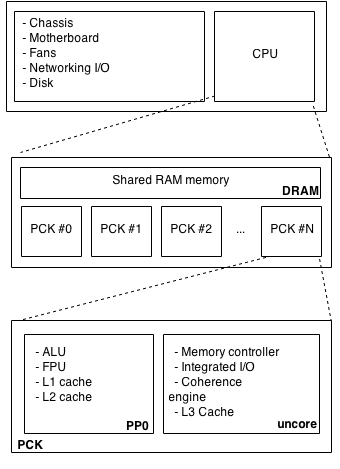
\includegraphics[width=75mm]{img/energy_model.png}
\caption{Components that contribute for power consumption in HPC. Taken from \cite{ACAT}}
\label{fig:power-consumption-model}
\end{figure}

\section*{Tools for measuring energy consumption}

\subsection{Internal tools}

\subsubsection*{Running Average Power Limit}
%internal tools
%RAPL
Recent Intel boards provide a powerful way to measure fine grained energy consumption of their CPUs with the Running Average Power Limit (RAPL) technology. RAPL has been included on the SoC from the factory since the Sandy Bridge family of processors.

Contrary to other solutions (such as TI INA231, for example), which are implemented as discrete
chips, RAPL is embedded as part of the CPU package itself and
provides information on the CPUs own subsystems. In particular RAPL
provides data for three different domains: \textbf{package} (pck),
which measures energy consumed by the system's sockets, \textbf{power
plane 0} (pp0), which measures energy consumed by the CPU core(s),
and \textbf{dram}, which accounts for the sum of energy consumed
by memory in a given socket, therefore excluding the on-core
caches~\cite{INTELMAN}. As for the discrete components case, the
timing resolution of measurements is in the millisecond range~\cite{RAPL1}.
This is fine enough to allow exploiting such data to build an energy
consumption sampling profiler for applications, similar to how performance
sampling profilers work (see section~\ref{sec:sampling}).
Finally, in addition to power
monitoring of the sockets, RAPL can limit the power consumed by the
different domains. This feature, usually referred as power capping,
allows the user to define the average power consumption limit of a
domain in a defined time window and allows more accurate independent
measurements of the non limited components.

\subsubsection*{TI INA 231}
There are chips that provide similar power monitoring capabilities than RAPL, but for any architecture and technology. An example is the Texas Instrument (TI) INA231 \cite{TIINA231}. The TI INA231 is a power monitor that reports current, voltage and power consumption of CPU, DRAM and cores of the SoC which is attached. Some vendors include the TI INA231 in their boards from origin, relying on an external technology to provide the same capabilities as RAPL monitoring.

Similarly to RAPL, the sampling resolution is high (at the sampling rate of microseconds) and the error is relatively low. On the other hand, the TI INA231 does not have capping capanilities.


\subsection{External tools}

There are different techniques and tools to measure the power consumed by the whole system ~\ref{fig:power-consumption-model}. Usually when the system is part of a server rack, the rack itself offers an API to sample the power consumed by each of the systems and overall rack power consumed. For simpler systems, it is recommended to use either power sockets with power meters or an external power meter. 

The resolution and errors of external tools vary according to their nature. The resolution can range from microseconds - when the sampling is done digitally - to seconds - when the sampling is done by a person. It is recommended to use API and digital based external tools in order to achieve the best resolution and error possible. 



\section*{Conclusion}
There are many different methodologies and tools to measure energy consumption of computing systems. The differences between the existent options range from granularity, accessibility, error and resolution and also from hardware or software approaches. The decision for which tools and techniques should be relied upon for the measurements is important when conducting research on energy efficiency. The decision is directly dependent on the goals of the experiment and the availability of the tools according to the technology to be used. 

Most of the techiques and tools outlined in this section were used in our experiments and are further discussed in the Experiments and Analysis chapters. In addition, the original paper which dwelves into the techniques and tools in more detail and was published at the ACAT'2014 conference proceding is attached as Appendix A. %done draft
 \chapter{Experiments}


During our research, we have performed several experiments under different
settings. The main goal was to understand how the ARM and Intel architectures
perform under authentic scientific computing workloads from an energy
consumption standpoint. Furthermore, our goal was to compare the results
obtained to evaluate the potential of ARM architectures to perform HPC tasks, in
comparison to the Intel architectures.
The software used to run or simulate authentic scientific computing tasks is
widely used in production and research at the CMS experience. We have used the
CMSSW framework [ref] (see section Y below) and ParFullCMS [ref] (see section X
below).  

We organized the experiments in 3 sets. The sets differ from methodology,
hardware and software used and general experimental conditions. However, the
main goal of such experiments is always the same: to understand if ARM
architectures have potential to replace Intel in scientific computing from an
energetic standpoint. The techniques and tools used to perform the energy
consumption measurements were based on the study presented on the previous
chapter. The setups of the experiments and tools used to perform the energy
measurements during the experiments are explained and detailed on section W.

The remainder of this chapter is organized as per set of experiment. For each
setup, we present the hardware and software setups and energy measurement tools
used. We will refer the batch of experiments as first (1SE), second (2SE) and
third (3SE) set of experiments throughout the rest of the document. 

\section{First set of experiments}
\section{Second set of experiments}

\begin{figure}[h!]
  \centering
    \includegraphics[width=100mm]{"img/machine_specs"}
    \caption{Specifications of the machines used in the 3SE}
    \label{fig:aalto_quad_clamp}
\end{figure}

\section{Third set of experiments}


 %done draft
 %%%%%\chapter{Results}

This chapter presents the results of the experiment descibed in the later chapter. The plots and figures in this chapter can be divided into 3 sections. The first section outlines the results of the first set of experiments. The second section outlines the results of the second set of experiments. The last section outlines the results that aim at studying the CMSSW framework is a Non-Uniform Memory Access (NUMA) environment.

In the next chapter, we analyse the results based on the content of this chapter.

%full results
\begin{figure}[h!]
  \centering
    \includegraphics[width=100mm]{"img/aalto/aalto_total_quad"}
    \caption{All stages of the CMSSW experiments on Intel\_quad}
    \label{fig:aalto_quad_clamp}
\end{figure}

\begin{figure}[h!]
  \centering
    \includegraphics[width=100mm]{"img/aalto/aalto_total_atom"}
    \caption{All stages of the CMSSW experiments on Intel\_atom}
    \label{fig:aalto_atom_clamp}
\end{figure}

\begin{figure}[h!]
  \centering
    \includegraphics[width=100mm]{"img/aalto/aalto_total_arm"}
    \caption{All stages of the CMSSW experiments on ARM\_viridis}
    \label{fig:aalto_arm_clamp}
\end{figure}



%event processing stage
\begin{figure}[h!]
  \centering
    \includegraphics[width=100mm]{"img/aalto/aalto_quadEvents"}
    \caption{CMSSW experiments on Intel\_quad - event processing stage}
    \label{fig:aalto_quad_events}
\end{figure}

\begin{figure}[h!]
  \centering
    \includegraphics[width=100mm]{"img/aalto/aalto_atomEvents"}
    \caption{CMSSW experiments on Intel\_atom - event processing stage}
    \label{fig:aalto_atom_events}
\end{figure}

\begin{figure}[h!]
  \centering
    \includegraphics[width=100mm]{"img/aalto/aalto_armEvents"}
    \caption{CMSSW experiments on ARM\_viridis - event processing stage}
    \label{fig:aalto_arm_events}
\end{figure}



%time comparison
\begin{figure}[h!]
  \centering
    \includegraphics[width=100mm]{"img/aalto/aalto_all_time"}
    \caption{Processing time comparison}
    \label{fig:aalto_time}
\end{figure}

%final results
\begin{figure}[h!]
  \centering
    \includegraphics[width=150mm]{"img/aalto/aalto_all_results"}
    \caption{Energy efficiency comparison for the first set of experiments - External measurements}
    \label{fig:aalto_all_results}
\end{figure}


%ParFullCMS
\begin{figure}[h!]
  \centering
    \includegraphics[width=150mm]{"img/acat/results1"}
    \caption{Multithreaded ParFullCMS comparison between Intel\_xeon and ARM\_odroid}
    \label{fig:parfull_results}
\end{figure}

\begin{figure}[h!]
  \centering
    \includegraphics[width=100mm]{"img/aalto/parfull_results_aalto"}
    \caption{Multithreaded ParFullCMS comparison between Intel\_xeon, ARM\_viridis and ARM\_odroid}
    \label{fig:parfull_results_aalto}
\end{figure}


%RAPL measurements example
%\begin{figure}[h!]
%  \centering
%    \includegraphics[width=150mm]{"img/cern/rapl"}
%    \caption{RAPL measurements with different load combinations }
%    \label{fig:RAPL table}
%\end{figure}



%NUMA and CMSSW
\begin{figure}[h!]
  \centering
    \includegraphics[width=150mm]{"img/numa/16proc_no_binding"}
    \caption{RAPL measurements of NUMA nodes - 16 processes with no explicit
    \label{fig:nf_ss}
binding}
\end{figure}

\begin{figure}[h!]
  \centering
    \includegraphics[width=150mm]{"img/numa/16proc_node2and3"}
    \caption{RAPL measurements of NUMA nodes - 16 processes. Explicit binding
    \label{fig:nf_ss}
on node \#2 and node \#3 binding}
\end{figure}

\begin{figure}[h!]
  \centering
    \includegraphics[width=150mm]{"img/numa/32proc"}
    \caption{RAPL measurements of NUMA nodes - 32 processes with no explicit
    \label{fig:nf_ss}
binding}
\end{figure}

\begin{figure}[h!]
  \centering
    \includegraphics[width=150mm]{"img/numa/32proc_explicitly_distributed"}
    \caption{RAPL measurements of NUMA nodes - 32 processes. Processes
distributed evenly explicitly - 8 processes per node. }
    \label{fig:nf_ss}
\end{figure}




 \chapter{Analysis}



In this chapter, we present our analysis based on the results shown in the last chapter. The scope of the analysis presented in this section is twofold: to compare the
platforms from an energy efficiency perspective and analyze the tools and techniques used on the different experiment sets. 


The first section and second section of this chapter analyse the different tools and techniques used
to perform the experiments, as well as the results itself. The first section analyses the 1SE, whereas the second section is dedicated to analyse the 2SE. As stated before, the difference between 1SE and 2SE has to do with the machine setups and the tools used to measure the energy consumed. The data and results of the experiments are shown along the analysis.

In the final of this section, we outline the highlights of the analysis for
each set of experiments.

\section{First Set of Experiments}

\begin{figure}[h]
  \centering
    \includegraphics[width=100mm]{"img/aalto/aalto_total_quad"}
    \caption{All stages of the CMSSW experiments on Intel\_quad}
    \label{fig:aalto_quad_clamp}
\end{figure}



In figures~\ref{fig:aalto_quad_clamp}, ~\ref{fig:aalto_atom_clamp} 
and~\ref{fig:aalto_arm_clamp} it is plotted the energy measurements from the beginning until the end of the event generation-simulation by the CMSSW. The energy measurements were done using a meter clamp. The energy measured is represented in the Y-axis and the X-axis represents the time of the experiment in samplings. For each experiment, a sample corresponds to the same time.

In the figures ~\ref{fig:aalto_quad_events}, ~\ref{fig:aalto_atom_events} and ~\ref{fig:aalto_arm_events}, we trimmed out the initialization stage and connection stage of the workload and only show the event processing stage. Whereas the Y-axi represents the energy measured in Watts, the X-axis represents the time spent until the correspondent energy sampling.

Finally, the figures ~\ref{fig:aalto_time} and ~\ref{fig:aalto_efficiency_comparison} compare the time spent by each of the hardware setups to process the workflow and the power consumption efficiency of the different setups, respectively.

\begin{figure}[h]
  \centering
    \includegraphics[width=100mm]{"img/aalto/aalto_total_atom"}
    \caption{All stages of the CMSSW experiments on Intel\_atom}
    \label{fig:aalto_atom_clamp}
\end{figure}



\subsubsection*{CMSSW stages}

\begin{figure}[h]
  \centering
    \includegraphics[width=100mm]{"img/aalto/aalto_total_arm"}
    \caption{All stages of the CMSSW experiments on ARM\_viridis}
    \label{fig:aalto_arm_clamp}
\end{figure}

Based on the figures~\ref{fig:aalto_quad_clamp}, ~\ref{fig:aalto_atom_clamp} 
and~\ref{fig:aalto_arm_clamp}, we can distinguish three different patterns of energy consumption during the expriement. 
We refer to each pattern as being part of a different CMSSW stage. The stages can be better identified 
when plotting the memory workload and the CPU usage (see ~\ref{fig:memory_stages}).

\begin{figure}[h]
  \centering
    \includegraphics[width=100mm]{"img/aalto/memory_stages"}
    \caption{Memory usage during the 3 different stages}
    \label{fig:memory_stages}
\end{figure}

The first stage consists is the initialization process. During this stage, the memory is the main module being used and thus, it is out od the scope of this work to analyse this stage in depth. 

The second stage is the connection phase. The goal of this stage is to fetch the metadata from
the CERN servers that allow the event generation-simulation. The metadata is needed to perform the reconstruction of the events. Once again, 
during this stage the CPU load is low when compared to the memory workload. 

The third stage corresponds to the event processing. This last stage is CPU intensive and it has the most relevant data to to our study, since we our goal is to compare the energy efficiency of the different CPUs. The event processing stage alone is represented by 
the figures ~\ref{fig:aalto_quad_events}, ~\ref{fig:aalto_atom_events} and ~\ref{fig:aalto_arm_events}.

\begin{enumerate}
\item Add memory plots? -- easier to identify the 3 stages but out of scope
\end{enumerate}

%event processing stage
\begin{figure}[h]
  \centering
    \includegraphics[width=100mm]{"img/aalto/aalto_quadEvents"}
    \caption{CMSSW experiments on Intel\_quad - event processing stage}
    \label{fig:aalto_quad_events}
\end{figure}

\begin{figure}[h]
  \centering
    \includegraphics[width=100mm]{"img/aalto/aalto_atomEvents"}
    \caption{CMSSW experiments on Intel\_atom - event processing stage}
    \label{fig:aalto_atom_events}
\end{figure}

\begin{figure}[h]
  \centering
    \includegraphics[width=100mm]{"img/aalto/aalto_armEvents"}
    \caption{CMSSW experiments on ARM\_viridis - event processing stage}
    \label{fig:aalto_arm_events}
\end{figure}

\subsubsection*{Relative importance of the stages}
The most important stage when studying the energy efficiency of
workload with the CMSSW is the last stage. There are three main reasons for that: Firstly, the CMSSW configuration at CERN has caches that speed up considerably the second stage [refs], thus reducing the energy consumed in the connection stage.
Secondly, the first and second stages are not CPU intensive.
Lastly, the processing stage is the only one that the energy consumption is directly porpotional o the amount of events. Therefore, given any large amount of
data to be processed, the last stage will consume so much more energy than the former stages that the first two stages will become irrelevant in terms of overall energy consumption. Therefore, we focus our energy consumption analysis on the event processing stage only. The event processing stage alone is represented by the figures ~\ref{fig:aalto_quad_events}, ~\ref{fig:aalto_atom_events} and ~\ref{fig:aalto_arm_events}


\subsubsection*{Overcommiting CPU and energy efficiency}
We consider a CPU to be overcommited when it has to process more threads or processes than the physical cores available.

If we consider each hardware setup individually, the time needed for running the three stages of the experiment is roughly the same, if the CPU is not overcommitted. When
the number of processes exceed the number of available cores, the time to 
process the events increases since there are no available cores to process the
events concurrently. In the overcommitted situation, the time increase follows
the ratio \textit{nr\_of\_processes/nr\_of\_cores\_available}. 
For example, if the
number of processes running is 6 and the number of cores available is 4, the
time needed to process the events increases roughly 2/3 compared to when the
CPU is not overcommitted.

In terms of energy consumed by the CPU, we do not find any outstanding difference in terms of overall energy efficiency by comparing CPUs that are overcommited vs non overcommited, as we can seen in the Figure ~\ref{fig:aalto_all_results}. However, we expect that if the ratio \textit{nr\_of\_processes/nr\_of\_cores\_available} is large enough, it can affect negatively the energy performance given the energy overhead spent when the jobs are being swapped.


\subsubsection*{Time comparison}
When comparing the time taken by the different architectures to process the same
task (Figure ~\ref{fig:aalto_time}), the pattern is evident. 
Regardless the number of processes, the 
Intel\_quad architecture is faster than Intel\_atom and ARM\_viridis and ARM\_viridis is faster than Intel\_atom.
This fact is due to the architectures characteristics and its specifications, most notably the CPU clock speed.\\

%time comparison
\begin{figure}[h]
  \centering
    \includegraphics[width=100mm]{"img/aalto/aalto_all_time"}
    \caption{Processing time comparison}
    \label{fig:aalto_time}
\end{figure}


\subsubsection*{Energy efficiency comparison}
Given the metrics used in this study (see Metrics section in the Experiments chapter), it is clear that  
systems are  proportionally energy efficient with its ratio performance per 
watts. Therefore, by analyzing the Figure~\ref{fig:aalto_all_results}, it is evident that given the architectures and its configurations, ARM architecture outperforms in terms of energy efficiency its concurrence in all considered 
scenarios. In addition, we conclude that between Intel architectures, Intel\_atom is more energy efficient than the Intel\_quad. 

%final results
\begin{figure}[h]
  \centering
    \includegraphics[width=150mm]{"img/aalto/aalto_all_results"}
    \caption{Energy efficiency comparison for the first set of experiments - External measurements}
    \label{fig:aalto_all_results}
\end{figure}

%% tools and techniques
\subsubsection*{Measuring tools: external monitoring}
For this set of experiments, the external samples were acquired and recorded 
manually. This factor had a visible impact on the resolution of the measurements. Clearly,
the all the plot show spikes and rough transitions between samples. Moreover, the error
tends to increase proportional to the human interaction with the experiment. 
Therefore, we conclude that it is more effective to use digital and automated ways to sample and
log the data acquired during the measurements.

\subsubsection*{Measuring tools: software-based monitoring}
We used software mesaurement tools to get an estimated energy consumption by the memory and other system components. In this particular set of experiments, the memory energy measurements done with software were
of particular help to distinguish the different stages, which existence was
unknown before the experiment. The software-based tools can be used as a 
decision support and for learning about unknown and unexpected system behaviours. Thus, even if the output
does not directly show information about energy consumption of the system, it
can be important to support and explain expected - and unexpected - behaviors.
  

\section{Second Set of Experiments}
\subsubsection*{Energy efficiency comparison between Intel\_xeon and ARM\_odroid}

%ParFullCMS
\begin{figure}[h]
  \centering
    \includegraphics[width=150mm]{"img/acat/results1"}
    \caption{Multithreaded ParFullCMS comparison between Intel\_xeon and ARM\_odroid}
    \label{fig:parfull_results}
\end{figure}

In the Figure~\ref{fig:parfull_results}, we can see the energy efficiency comparison of Intel\_xeon and ARM\_odroid. The righmost plot represents the internal energy measurements, whereas the leftmost plot represents the external energy measurements. As in other energy efficiency comparisons in this study, we used the metrics \textit{nr\_of\_events/s/W} to represent the energy performance of the measured systems. 


\begin{figure}[h]
  \centering
    \includegraphics[width=100mm]{"img/aalto/parfull_results_aalto"}
    \caption{Multithreaded ParFullCMS comparison between Intel\_xeon, ARM\_viridis and ARM\_odroid}
    \label{fig:parfull_results_aalto}
\end{figure}

The main conclusion from ~\ref{fig:parfull_results} is that ARM\_odroid outperforms Intel\_xeon in both internal energy efficiency and external energy efficiency.

\subsubsection*{Energy performance and overcommited CPUs}

It is noticeable that ARM\_odroid has a significant energy performance decline when its cores are overcommited. It is also interesting to see that the energy performance decline in the ARM\_odroid is relatively larger on the internal energy measurements. One of the reasons we found in our raw results to explain this phenomenona is the large increase of time taken to process the events when the cores are overcommited. Thus, even if the cores are consuming the same Watts per second during the event processing stage, the energy efficiency will decrease with the time taken to process the events.  

On the other hand, the energy performance of Intel\_xeon does not seem to be significantly affected when overcommited. This phenomenon is explain by the fact that Intel\_xeon took roughly the same time to process the events when using one core per event and half a core per event.

We believe that the different results between ARM\_odroid and Intel\_xeon discussed below are due to the fact that ARM\_odroid is a development board and it does not implement sophisticated techniques such as Hyper Threading Technology (HTT) by Intel \cite{HTT}. According to Intel, HTT delivers two processing threads per physical core, which allows highly threaded applications to be processed faster. It is expected that if the ratio of  \textit{nr\_of\_threads/core} would be larger than 2, energy efficiency of Intel\_xeon would start to decline.  

We believe that if we would overcommit Intel\_xeon with more than 4 threads per core, the time to process the workload would increase, which would be followed by a degradation of energy performance.

\subsubsection*{Measurement tools and techniques}

The internal measurement tools used in ARM\_odroid and Intel\_xeon provide a fine grained resolution to the core level. The TI INA231 and RAPL chips can isolate the pp0, which consists of ALU, FPU, L1 cache and L2 cache when performing energy measurements. 

On the other hand, as stated in \cite{IPMI_resolution}, the lower resolution that IPMI tools offers for internal measurements include energy consumed by the 0P9V, 1P8V, VDD and Vcore rails, which includes the system on the chip, DRAM, Temperature Sensors, and ComboPHY Clock. The components that are measured by the IPMI tools at each energy sample are shown in the Figure \ref{fig:power_node_ipmitool}.

As a result of this measurement discrepancy, ~\ref{fig:parfull_results_aalto} shows that ARM\_viridis performs worse than any other machine. We believe that this result can be misleading, due to the fact that the tools used to measure the energy consumed by each of the setups measure different components in the CPU. We believe that if components measured in the ARM\_viridis would be same as the components measured on the ARM\_odroid and Intel\_xeon measurements, we would obtain a different result. Namely that ARM\_viridis would, at least, perform better that Intel\_xeon from an energy consumption perspective. Given the actual setup, we can not scientifically directly compare the results.

\begin{figure}[h!]
  \centering
    \includegraphics[width=150mm]{"img/aalto/power_node_ipmitool"}
    \label{fig:power_node_ipmitool}
    \caption{Representation of the Power Node measured by IPMI tools [make one myselfd and change!]}
\end{figure}


\subsection*{Comparison between First set of experiments and Second set of experiments}

When we compare the main results of the 1SE (Figure ~\ref{fig:parfull_results_aalto}) and 2SE (Figure ~\ref{fig:parfull_results}) we may be inclined to conclude that the setups in the 2SE presented an overall more efficiency than the setups the 1SE. Again, the used measurement tools play an important role and should not be disregarded when analysing the results. 
In the 1SE, we only performed external measurements. Thus, we discard the possibility to compare the 1SE results with the results of the internal measurements of the 2SE. 
As for the external measurements performed in both set of experiments, the tools for measuring the energy consumption of both experiments have disctinct resolution and grain. In the 1SE, we used the clamp meter for measurements in all setups. As for the 2SE, we used embeeded and computer-assisted tools to perform the external measurements. This discrepancy of tools, its resolutions and errors, make it difficult to compare the results of the 1SE and 2SE.

However, we can conclude that ARM architecture outperforms the Intel architectures in each and every experiment, regardless the measurement tools and methodologies used.

\section{Conclusions}
The main conclusion of our experiments is that given the setups used in our study, the ARM chipset Intel in terms of energy efficiency in every experiment.

We learned that the gen-sim mode of CMSSW has different stages and the most relevant from an energy consumption point of view is the latest one, when the events are processed.


In addition, we leanerd that the tools used to make the experiments play a crucial role in the whole experiment. It is important to assure that the measurement tools and methodologies in use are compatible and suitable to produce results that can be compared. This aspect can be hindered based on the availability of hardware and measurement tools. 

 cite\chapter{HTC in a dynamic energy pricing market}

One of the ways to utilize the conclusions from the experiments conducted in this study is to actively lower the energy bill in HTC. One approach could be to schedule jobs between more energy efficient but slower ARM architectures and the less energy efficient but faster Intel machines. This approach makes sense in a multi energy price ecosystem. A multi energy price ecosystem is an energy market where the prices float according to the overall power grid usage.

In this chapter, we present a study about the potential of an algorithm that schedules workload to machines with different energy and computation performance, based on the the daily dynamics of energy price. The main goal is to leverage computing heterogeneity to achieve the optimal ratio between work produced and price paid.  

\section{Dynamic electricity pricing model}

\begin{figure}[hours]
  \centering
    \includegraphics[width=100mm]{"img/pricing_model_table"}
    \caption{Examples of dynamic power energy pricing in different markets}
    \label{fig:pricing_model_table}
\end{figure}

We will use a simplified dynamic pricing model based on the empirical research of such models in real power grids. Based on some examples obtained, we can conclude that not all the countries adopt a dynamic electricity pricing model ~\ref{fig:pricing_model_table}. For the sake of this study, we will consider a hypothetical case where the dynamic pricing model works as in ~\ref{fig:pricing_model}. The red line in ~\ref{fig:pricing_model} represents the electricity price along the day. For the sake of simplicity, during this study we define that the price of electricity can is  60 euros/Mwh during 12 hours per day and 20 euros/Mwh during the remaining 12 hours of the day.  
	
As we can see based on the ~\ref{fig:pricing_model} and ~\ref{fig:pricing_model_table}, our simplified energy model presents a similar pattern to the energy prices of some countries.

\begin{figure}[h]
  \centering
    \includegraphics[width=150mm]{"img/pricing_model"}
    \caption{Simplified pricing model based on the Germany energy market}
    \label{fig:pricing_model}
\end{figure}

\section{Scheduling algorithm}

\subsection*{Problem formulation}

The main goal of the algorithm is to lower the electric bill in dynamic electricity markets. The algorithm schedules HPC workload among nodes with different energy profiles, depending the energy price at the time. In addition, the algorithm should ensure that a certain minimum amount of workload is processed. Thus, the algorithm input can be defined as (see also ~\ref{fig:input}): 

\vspace{10mm}

\textbf{Energy profile of the machines:}
\begin{itemize}
  \item[] Energy efficiency of the machines (ev/s/W);
  \item[] Time performance (ev/s);
\end{itemize}

\vspace{5mm}

\textbf{Computing requirements:}
\begin{itemize}
  \item[] Time deadline (s);
  \item[] Nr. events to be processed (ev);
\end{itemize}

\vspace{10mm}

Therefore, given a set of machines with different energy profiles; the computing requirements (how many events must be processed in how much time); and the energy pricing dynamics during 24h, \textit{what is the optimal machine scheduling that ensure the computing requirements and achieve the lowest price budget at the end of 24 hours} ?

\begin{figure}[h]
  \centering
    \includegraphics[width=150mm]{"img/input"}
    \caption{Example input for the scheduling algorithm}
    \label{fig:input}
\end{figure}


\subsection*{The scheduling algorithm}

\begin{figure}[h]
  \centering
    \includegraphics[width=150mm]{"img/scheduler_code"}
    \caption{Proposed scheduler algorithm written in Python}
    \label{fig:scheduler_code}
\end{figure}

The scheduling algorithm is presented in ~\ref{fig:scheduler_code}. For simplicity sake, the algorithm is written in Python.

The main idea behind the construction of the algorithm is that it should assign the maximum number of events to be processed to the lowest priced configuration possible, given the existent constrains (deadline). For example, if it is possible to process all the data only using the ARM architecture in the lowest and highest energy pricing times, then there is no need to use the Intel machines to process the data. This way it is possible to reach the optimal scheduling of processing power given a deadline and several machines with different configurations.

\subsubsection*{Algorithm walk-through}
The input of the algorithm are the number of days that we have to process the data (deadline); the number of events to process; and a set of buckets. We define a bucket as a tuple of \textit{ (machine, energy\_price\_level) }. The table ~\ref{fig:input_table} shows an example of what buckets can be.
The expected output os the final price of the scheduled processing. If the processing power of the data center is not enough to complete the task before the set deadline, the output will be an error.


\vspace{10mm}
Based on the code in ~\ref{fig:scheduler_code}: 
\begin{itemize}
  \item[\textbf{Line 5}] Sorts the buckets from lowest to highest price per event. The goal is to use the as much processing power of the cheaper buckets as possible.
  
  \item[\textbf{Line 7}] The algorithm goes through all the available buckets. It starts by considering the cheapest options and only uses the more expensive if needed.
  
  \item[\textbf{Line 11}] Ensures that the money spent by the last bucket will only take into consideration the events left. 
  
  \item[\textbf{Lines 14-15}] The money spent by a given bucket is the number of events processed times the price per event.
  
  \item[\textbf{Lines 18-20}] When there are no events left to process, finish the algorithm and calculates the final price (the sum of the money spent by all the buckets to compute the tasks)
  
  \item[\textbf{Lines 22}] After the buckets had all the events processed given the deadline, if there is still events left the algorithm throws an errors. In this case, more buckets have to be added of the deadline should be increased.

  \end{itemize}


\subsection*{Use case}

Let us consider the values presented in ~\ref{fig:input_table} as a case scenario to use the scheduling algorithm. The values presented show the energy profile of a hypothetical mini data center set up. The data center has only two machines: a ARMv7 and a Intel x86 server. The energy profile (number of events processed by day and energy consumed) is based on the values from the experiments analyzed in the previous chapters. The prices are based on the simplified dynamic energy pricing model of 60 euros/Mwh in the high pricing hours (comprised of 12h/day) and 20 euros/Mhw in the low pricing hours (comprised on 12h/day)

\begin{figure}[h]
  \centering
    \includegraphics[width=150mm]{"img/input_table"}
    \caption{Example input for the scheduling algorithm}
    \label{fig:input_table}
\end{figure}

Given the data in ~\ref{fig:input_table}, the algorithm should be started as in ~\ref{fig:scheduler_code_init}.

\begin{figure}[h]
  \centering
    \includegraphics[width=150mm]{"img/scheduler_code_init"}
    \caption{Start the algorithm programatically}
    \label{fig:scheduler_code_init}
\end{figure}

\vspace{10mm}

Given the input ~\ref{fig:scheduler_code_init} and the algorithm in ~\ref{fig:scheduler_code}, the result is that the optimal final price for computing 1200000 events in 2 days is 1.97125776 euros, where the ARM machine processed 204120 events in the low pricing window and 204120 in the high pricing window during the 2 days. As for the Intel machine, it had to process only 791760 events during the low pricing window. The Intel machine does not need to be working during the high pricing windows in order for the data center to meet the deadline.

\vspace{10mm}


We ran the scheduler algorithm with different deadlines to compare the final prices and how much work do the different machines have to perform in the different energy pricing window. The results are condensed in the  ~\ref{fig:prices_final_table}.

\begin{figure}[h]
  \centering
    \includegraphics[width=150mm]{"img/prices_final_table"}
    \caption{Algorithm results for different deadlines}
    \label{fig:prices_final_table}
\end{figure}


Based on the information of the table ~\ref{fig:prices_final_table}, if we the deadline is stricter, the price to pay will be bigger as expected. We can also conclude that the machines we have access to are not able to process the 1200000 events in 1 day only. As expected, the more time there is to process the events, the less the algorithm uses the most expensive buckets to process the data. When the deadline is 75 and 100 days, all the events are processed by the ARM machine during the time when the energy price is lower. Thus, this is the cheapest possible case given the data center setups and energy price model used in this use case.



\section{Further developments}

Well known algorithms such as job shop scheduling algorithm and others can be applied using the same rational. We expect that different algorithms present different results and that the nearly-optimal scheduling algorithm can be achieved with one well studied existing algorithm. We believe that to research heterogeneous HTC in a dynamic energy pricing market further on may present potential to unlock savings in energy budget for data centers. It would be interesting to apply several other scheduling algorithms to this scenario and compare the obtained results.

\section{Conclusions}

Our solution takes a different perspective when compared with related research. Studies conducted by Yan Wang, et al.  \cite{TASK_SCHED} and Guosun Zeng, et al. \cite{EXE_METHOD} do not take the
dynamics of electrical pricing into consideration. However, their algorithm is
already quite complex and proved NP-complete, to the point they have to come up
with heuristic algorithms to apply it in the real world.

Therefore, our approach may have some novelty in a really narrow and still
unexplored idea: to develop a scheduling algorithm for heterogeneous HPC that
takes into consideration the nodes' energy profile, the dynamic electricity
price and also, eventually, the tasks' energy profiling. The algorithm would
schedule the jobs in order to minimize the energy consumption and energy bill
(note: energy consumption and energy bill are not the same thing), while the
deadline is met. 

However, there are some open points that we still have might want to
consider. First, as Xu Yang, et al. \cite{DYN_PRICING_HPC} state, it is important to ensure
that the hardware existent in the data center is used at its full potential, in
order to not waste the investment made when it was purchased. Our solution,
though, does not insure that since the idea is to power down/idle machines that 
are less power efficient in high-peak times. Secondly, from a practical
perspective, if we consider only the scheduling between ARM and Intel architectures, 
it seems not likely that the data center will haver the same software running
over both architectures at the same time, give the expertise and investment
needed to have the application stack running properly in both architectures (as
we witness with CERN's efforts). If we decide to abstract from that point and
see the machine's architectures as a black box, then that's not a problem. Thirdly, 
comparing with other recent research works
such as the one conducted by Yan Wang, et al. \cite{TASK_SCHED}, our algorithm model seems to be over simplifying the
problem to an extent that might hinder our purposes of creating a practical and
energy efficient scheduling algorithm for heterogeneous HPC under dynamic
electrical pricing.

Our solution is a starting point for a deeper study of heterogeneous computing applied to HTC in a dynamic energy pricing market. We used the data and experiments obtained in the previous chapters of this study to test our algorithm in a scenario as closest to the reality as possible. Based on the budget savings shown in the results, our approach shows potential to be used in a production scenario. %done draft
 \chapter{Future Work}

From the experiments perspective, we believe that it would be valuable to run more experiments in environments closer to production than development boards. The output of such experiments would present valuable complementary data to what we have got. Another interesting research work would be to understand if the drawbacks of the approach make it inviable in a real production scenario.


In addition, to run more experiments using a methodology where the tools and techniques are as accurate as possible (based on the learning of Chapter 3) and where the results can be compared across all the experiments. This might be difficult to achieve given the different tools available to measure in the different platforms. Another interesting research subject would be to develop a cross platform and accurate way to perform high resolution power consumption measurements. In addition, it would be interesting to develop accurate mathematical models of energy consumption by data centers consisting of heterogeneous (RISC and CISC) processing nodes.


It would be interesting to develop further the scheduling algorithm for dynamic electricity markets and HTC presented in the Chapter 6. In addition, to apply the same idea to different well known scheduling algorithms. Also, to improve the energy model used and increase the complexity of the energy profiles in order to the results to be as close to the reality as possible. Another interesting research work would be to understand if the drawbacks of the approach taken make it inviable to use in a real production scenario.

 %done draft
 \chapter{Conclusions}

Energy consumption has has become a major bottleneck in HTC and scientific computing, where the amount of data to analyse has been increasing manyfold every year. Besides the economical issues of the increasing energy consumption, social and environmental concerns should be also considered. Therefore, to research how to build and develop energy efficient HTC systems has become of paramount importance among the research community.

The goal of this research was to understand wheter RISC architectures are capable of improving the energy efficiency of scientific computing without performance degradation, when compared with the current x86 Intel architectures.

In order to achieve that goal, we conducted reasearch on tools and techniques for measuring energy consumption at different system levels. In addition, we conducted experiments that aimed at comparing the energy performance of ARM and Intel architectures, working under real world workloads and frameworks. Finally, we used the results of the experiments to develop a scheaduling algorithm that optimizes the eletricity bill of heterogeneous data centers working in a dynamic eletricity pricing markets. 

\vspace{5mm}

Our main contribuitions are: 

\begin{itemize}
  \item We researched and outlined best practives for different system levels. The results of this work were published in the conference proceedings of the 16th International workshop on Advanced Computing and Analysis Techniques in physics research (ACAT'2014). The article was called \textit{Techniques and tools for measuring energy efficiency of scientific software applications}

  \item Our experiments and research shown that ARM architecture shows potential for an energy savings in HTC when compared to the x86 systems widely used nowadays. 

  \item Our research shown that heterogeneous computing can be leveraged in HTC in markets where the price of the eletricity is dynamic. We shown how to achieve savings in such environment and developed a scheaduling algorithm that accomplishes that.
\end{itemize}
 %done draft
 %\documentclass[a4paper]{jpconf}
\usepackage{graphicx}
\usepackage{lineno}
\usepackage{hyperref}

\begin{document}
%\linenumbers

\title{Techniques and tools for measuring energy efficiency of scientific software applications}

\author{David Abdurachmanov$^1$, Peter Elmer$^2$, Giulio Eulisse$^3$, Robert Knight$^4$, Tapio Petteri Niemi$^5$, Jukka Nurminen$^6$, Filip Nyback$^6$, Goncalo Marques Pestana$^6$, Zhonghong Ou$^6$}

\address{$^1$ Digital Science and Computing Center, Faculty of Mathematics and Informatics, Vilnius University, Vilnius, Lithuania}
\address{$^2$ Department of Physics, Princeton University, Princeton, NJ 08540, USA}
\address{$^3$ Fermilab, Batavia, IL 60510, USA}
\address{$^4$ Research Computing, Office of Information Technology, Princeton University, Princeton, New Jersey 08540, USA}
\address{$^5$ Helsinki Institute of Physics, PO Box 64, FI-00014, Helsinki, Finland }
\address{$^6$ Aalto University, PO Box 11100, 00076 Aalto, Finland}

\ead{Peter.Elmer@cern.ch}

\begin{abstract}
As both High Performance Computing (HPC) and High Throughput Computing
(HTC) are sensitive to the rise of energy costs, energy-efficiency
has become a primary concern in scientific fields such as High
Energy Physics (HEP). There has been a growing interest in utilizing
low power architectures, such as ARM processors, to replace traditional
Intel x86 architectures. Nevertheless, even though such solutions
have been successfully used in mobile applications with low I/O and
memory demands, it is still unclear if they are suitable and more
energy-efficient in the scientific computing environment. Furthermore,
there is still lack of tools to derive and compare power consumption
for these types of workloads, and eventually to support software
optimizations for energy efficiency.

To that end, we have performed several physical and software-based
measurements of workloads from CERN running on ARM and Intel
architectures, to compare their power consumption and performance.
We leverage several profiling tools to extract different aspects
of the experiments, including hardware usage and software
characteristics. We report the results of these measurements and
the experience gained in developing a set of measurement techniques
and profiling tools to accurately assess the power consumption for
scientific workloads. [Version of~\today]
\end{abstract}

\section{Introduction}

 The most recent scientific applications have to process and store considerable 
volume of data. It is foreseeable that the volume of data will increase 
considerably in the future, as technology and requirements enhance. Thus, energy 
consumption has become a major concern amongst the scientific community. \\
 The Large Hadron Collider (LHC) ~\cite{LHCPAPER} at the European Laboratory for 
Particle Physics (CERN) in Geneva, Switzerland, is one of the scientific
projects which computational requirements are too massive for resources to be
 processed and held in one single infrastructure. Hence, data processing and 
storage 
are distributed across the Worldwide LHC Computing Grid (WLCG) ~\cite{WLHC}, 
which uses resources from 160 computer centers in 35 countries. The access to 
such computational resources have made possible CMS ~\cite{CMSDET} and ATLAS
 ~\cite{ATLAS} experiments to achieve important results, such as the discover of 
the Higgs Boson ~\cite{CMSHIGGS, ATLASHIGGS}. While enabling this and other
discoveries, the WLHC consumes massive amount of computational resources and, 
proportionally, energy. Only CMS experiment used approximately 80,000 to 100,000 
x86-64 cores of capacity in 2012, according to ~\cite{ACAT13ARM, CHEP13ARMPHI}.
In the future, with the improvement of the detector's luminosity, the dataset size
will increase by 2-3 orders of magnitude ~\cite{ACAT13ARM, CHEP13ARMPHI},
presenting even more challenges from the energy consumption point of view. \\

 In order to find and develop better solutions to improve energy efficiency in
High Energy Physics (HEP), it is
 important to understand how energy is used by the HEP systems themselves. There 
are 
few tools and techniques that facilitate researchers to reach that goal. Some of
these tools and techniques are outlined and described in this article.  \\
 As energy efficiency becomes a concern, new
solutions have been considered to develop energy efficient systems. One potential
solution is to replace the traditional Intel x86 architectures by low power
architectures such as ARM. A comparison of the energy efficiency between ARMv7 and 
x86 Intel architecture is conducted in this article. The experiments use CMS 
workloads and rely on the techniques and tools described earlier to perform the
measurements.\\

This article is structured as following. Firstly, we describe where is energy consumed in a HTC system. Secondly, we outline some of the tools and techniques available to measure and monitor energy consumption on HTC systems. Finally, we present the results of a comparison between ARMv7 and Intel Xeon architecture using CMS workloads.


\section{Tools and techniques for energy measurement}

important to know where is energy consumed and what tools and techniques are available to do so

\begin{figure}[ht!]
\centering
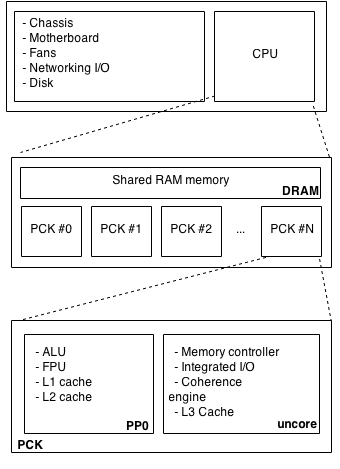
\includegraphics[width=70mm]{img/energy_model.png}
\caption{Components that contribute for power consumption in HPC}
\label{overflow}
\end{figure}

\subsection{External probing devices}

\subsubsection{Noninvasive clamp meters}
\subsubsection{Power distribution units}

\subsection{Internal probing chips}
What is it ? Refer to figure above in order to mention which machine components do the internal probing chips  monitor

\subsubsection{Running Average Power Limit}
Running Average Power Limit (RAPL) provides a platform for monitoring and limiting power of  systems on chip (SoC). It is a Intel's technology which was introduced initially on the Sandy Bridge processors. RAPL platform exposes on-chip measurements via the MSR registers. According to ~\cite{RAPL1}, this technology offers power measurements of the system at a granularity impossible to reach before with other tools.

As documented by Intel in ~\cite{INTELMAN}, there are 3 different domains to sample energy consumed by different SoC components on a server. The domains are: package (accounting for the entire socket), power plane 0 or pp0 (accounting for energy consumed by the core) and dram (sum of energy consumed by memory in a given socket, excluding the core caches). The measurements are dumped in the MSR registers at a frequency of ~1 kHz and are exposed to the user via /dev/cpu/<cpu\_nr>/msr. It is also possible to read and write data from the MSR register using Intel’s open source tool msr-tools ~\cite{MSRTOOLS}. 

In addition to power monitoring of the sockets, it can limit the power consumed by the different domains. This feature, usually referred as power capping, allows the user to define the average power consumption limit of a domain in a defined time window. For more information about RAPL’s features and configurations, refer to section 14.9.1 of Intel’s Developer’s manual ~\cite{INTELMAN}.

- RAPL mode 0 vs RAPL mode 1 \\
"The DRAM RAPL is not enabled in BIOS by default. To enable in BIOS, go to Memory Configuration and change the mode from 'Performance' to 'Power Efficient'. Then select 'Mode 1'. This is the VR (voltage regulator) mode of power estimation. The accuracy of this mode is highly dependent on the OEM platform. For Intel reference platforms the accuracy of DRAM power estimation may produce up to ~30% error"


The advantages of using RAPL for measuring power consumption are a straightforward and already installed tool to perform fine grained measurements of energy consumption on SoC and its components.

On the other hand, the drawbacks are lack of documentation available about the monitoring chip. To the knowledge of the authors, specifications such as error degrees, accuracy and implementation diagrams are not publicly available. In addition, the RAPL technology is vendor locked. Considering those two points, it is difficult to accurately compare and reason power measurements between SoCs from Intel and other vendors.


\subsubsection{TI INA231 and alike}

\subsection{Software based measuring tools}
\subsubsection{powertop and alike}
\subsection{IgProf}
Filip's work \\


\section{Comparison of power efficiency of ARM and Intel}

 \subsection{Workflow and experiments setup}
    Description of the experiments done in ARM ({\it Cortex-A15 Quad and Cortex-A7 Quad 1.4GH}) and Intel ({\it Xeon E5-4650})

\subsection{ARM results}
    Result of measurements done in ARM


\subsection{Intel results}
    Result of measurements done in Intel


\subsection{Analisis}
    Analysis and comparison of above described experiments


\section{Conclusions}

\section*{Acknowledgements}
This work was partially supported by the National Science Foundation, under
Cooperative Agreement PHY-1120138, and by the U.S. Department of Energy.

\section*{References}

\bibliographystyle{unsrt}
\bibliography{acat2014-energy-efficiency}

\end{document}
 %done draft


% Load the bibliographic references
% ------------------------------------------------------------------
% You can use several .bib files:
% \bibliography{thesis_sources,ietf_sources}
\bibliography{sources}


% Appendices go here
% ------------------------------------------------------------------
% If you do not have appendices, comment out the following lines
\appendix
\chapter{First appendix}
\label{chapter:first-appendix}

This is the first appendix. You could put some test images or verbose data in an
appendix, if there is too much data to fit in the actual text nicely.



% End of document!
% ------------------------------------------------------------------
% The LastPage package automatically places a label on the last page.
% That works better than placing a label here manually, because the
% label might not go to the actual last page, if LaTeX needs to place
% floats (that is, figures, tables, and such) to the end of the 
% document.
\end{document}
